\section{完整实验配置、检查点与复现}\label{app:config}

\footnotesize
\setlength{\tabcolsep}{3pt}
\begin{longtable}{@{}p{0.13\linewidth}p{0.52\linewidth}p{0.27\linewidth}@{}}
\caption{配置与检查点事实。标「推算」的量为本文推算，其余引自团队实现文档与配置。}
\label{tab:config}\\
\toprule
项 & 值 & 备注 \\
\midrule
\endfirsthead
\multicolumn{3}{@{}l}{\tablename~\thetable\ （续）}\\
\toprule
项 & 值 & 备注 \\
\midrule
\endhead
\midrule
\multicolumn{3}{@{}r}{续下页}\\
\endfoot
\bottomrule
\endlastfoot
模型配置 & \texttt{GRIDMAN\_MEDIUM}：\texttt{embed\_dim}=1024，\texttt{blocks}=3，\texttt{patch\_size}=64（本文检查点 v\_0d3：\texttt{chunk\_size}=192；现行 v\_0d4 MEDIUM：\texttt{chunk\_size}=1，\texttt{bptt}=16） & 4 个 \texttt{c\_state} \\
实现版本 & 行为描述 v\_0d4（2026-10-18）；全部数字出自 v\_0d3 检查点，存档不互相兼容 & 见 \S\ref{sec:model} 表 \ref{tab:version} \\
参数量 & 437.8M & 权重 $+$ 状态合计 \\
词表 & 300（字节 0--255，\texttt{pad}=256，\texttt{eos}=257） & byte 级，无 OOV \\
状态规模 & batch$=1$ 切片合计 $14{,}072{,}832$ 个 fp32 元素（$\approx53.7$\,MiB）：\texttt{memory} $12{,}954{,}624$（$49.4$\,MiB）$+$ \texttt{MTM} $1{,}048{,}576$（$4.0$\,MiB）$+$ \texttt{queue} $65{,}536$（$0.25$\,MiB）$+$ \texttt{recurrent} $4{,}096$（$0.016$\,MiB） & 按 v\_0d4 \texttt{StateLayout} 实测 \\
训练 & AdamW $+$ cosine，clip $1.0$，bf16，lr $5\times10^{-4}$，\texttt{bptt}=4 patch（256 token） & 192 条并行永续流（v\_0d3 检查点口径） \\
检查点 & \texttt{gridman\_medium\_v\_0d3\_pretrain}，step $144{,}000/705{,}600$（20\%） & 唯一使用的权重 \\
\midrule
\multicolumn{3}{@{}l}{\textbf{数据}} \\
\midrule
预训练 & \texttt{pretrain.jsonl} $\approx9.5$\,GB，每行 \texttt{\{"text": ...\}} & 每条流 chunk $\approx49.4$\,MB \\
微调 & \texttt{sft.jsonl} $\approx14$\,GB，多轮对话（仅 assistant token 计 loss） & 用作跨域档 \\
已消费区 & 每条流前 $144{,}000\times64\,\mathrm{B}=9.2$\,MB & 推算 \\
held-out 取行 & 每条流 chunk 内偏移 $\ge20$\,MB & 零污染 \\
\midrule
\multicolumn{3}{@{}l}{\textbf{复现：脚本 $\to$ 实验}} \\
\midrule
\texttt{common\_eval.py} & 脚手架：模型单例、teacher-forced 流式评测、文本源、组件手术 & 全部实验共用 \\
\texttt{a1\_hot\_vs\_blank.py} / \texttt{a1\_clean\_heldout.py} & A1（\S\ref{sec:a1}） & 后者为对齐窗口版 \\
\texttt{stage1\_a2\_a3\_a5.py} & A2、A3、A5（\S\ref{sec:a2}、\S\ref{sec:a3}、\S\ref{sec:s1-attr}） & \\
\texttt{stage1b\_a6.py} & A6 组件冻结（\S\ref{sec:s1-attr}） & \\
\texttt{stage2\_d1\_d2.py} / \texttt{stage2b\_d1\_d2.py} / \texttt{stage8\_d2b.py} & D1、D2、D2b（附录 \ref{app:dline}） & 2b 为 5-seed 修订版 \\
\texttt{stage3\_e1\_e5\_b2.py} / \texttt{stage6\_g1c\_e1long.py} & E1、E5、B2（\S\ref{sec:b1}、\S\ref{sec:b2}） & 含 512\,KB 长流 \\
\texttt{stage4\_g1\_g2.py} & G1a、G1b、G2（附录 \ref{app:g}） & \\
\texttt{stage5\_c1\_e2.py} & C1（作废，附录 \ref{app:c1}）与 E2（附录 \ref{app:eline}） & \\
\texttt{stage7\_b2\_freeze.py} & B2-freeze 组件归属（\S\ref{sec:b2}） & \\
\texttt{make\_figures.py} / \texttt{make\_fig\_a1.py} & 全部图表 & \\
\texttt{verify\_positions.py} & 模型无关回归自检（答案位置必须落在自己的 kv 块内） & 无 GPU 也可跑 \\
\end{longtable}
\setlength{\tabcolsep}{6pt}
\normalsize

\section{逐位置完整曲线}\label{app:curves}

正文引用的逐位置曲线：图 \ref{fig:a1}（A1 双曲线 $+$ 差值）、图 \ref{fig:a2}（A2 写入 vs 只读）、
图 \ref{fig:a3}（跨文档边界对齐恢复曲线）、图 \ref{fig:e1}（96\,KB 范数 $+$ per-position）、
图 \ref{fig:e5}（重置频率）、图 \ref{fig:e1long}（512\,KB 范数 $+$ 距离分桶）、
图 \ref{fig:b2} 与图 \ref{fig:b2freeze}（重复距离与组件归属）。
附录 \ref{app:eline} 给出污染自愈曲线（图 \ref{fig:e2}）。

\section{held-out 去污染统计}\label{app:decontam}

本文的 held-out 切分按「每条流 chunk 内偏移 $\ge20$\,MB」取行（\S\ref{sec:data}），
该偏移由「step $\times$ patch 长度 $=$ 9.2\,MB」推算得到，留有 $>2\times$ 余量。
B2 的分桶统计顺带产出了配对数量（表 \ref{tab:b2}），可作为分布性的旁证。
\pending{待补：与训练集（已消费区）的 4-gram 重叠率、以及 $n$-gram 去重后的行级去重率明细；
口径与实现见《论文大纲-B》第 1 章。}

\section{C 线与 E 线：遗忘、污染与稳定性}\label{app:cline}

\subsection{C1 受控遗忘曲线：作废说明}\label{app:c1}

\begin{figure}[H]
\centering
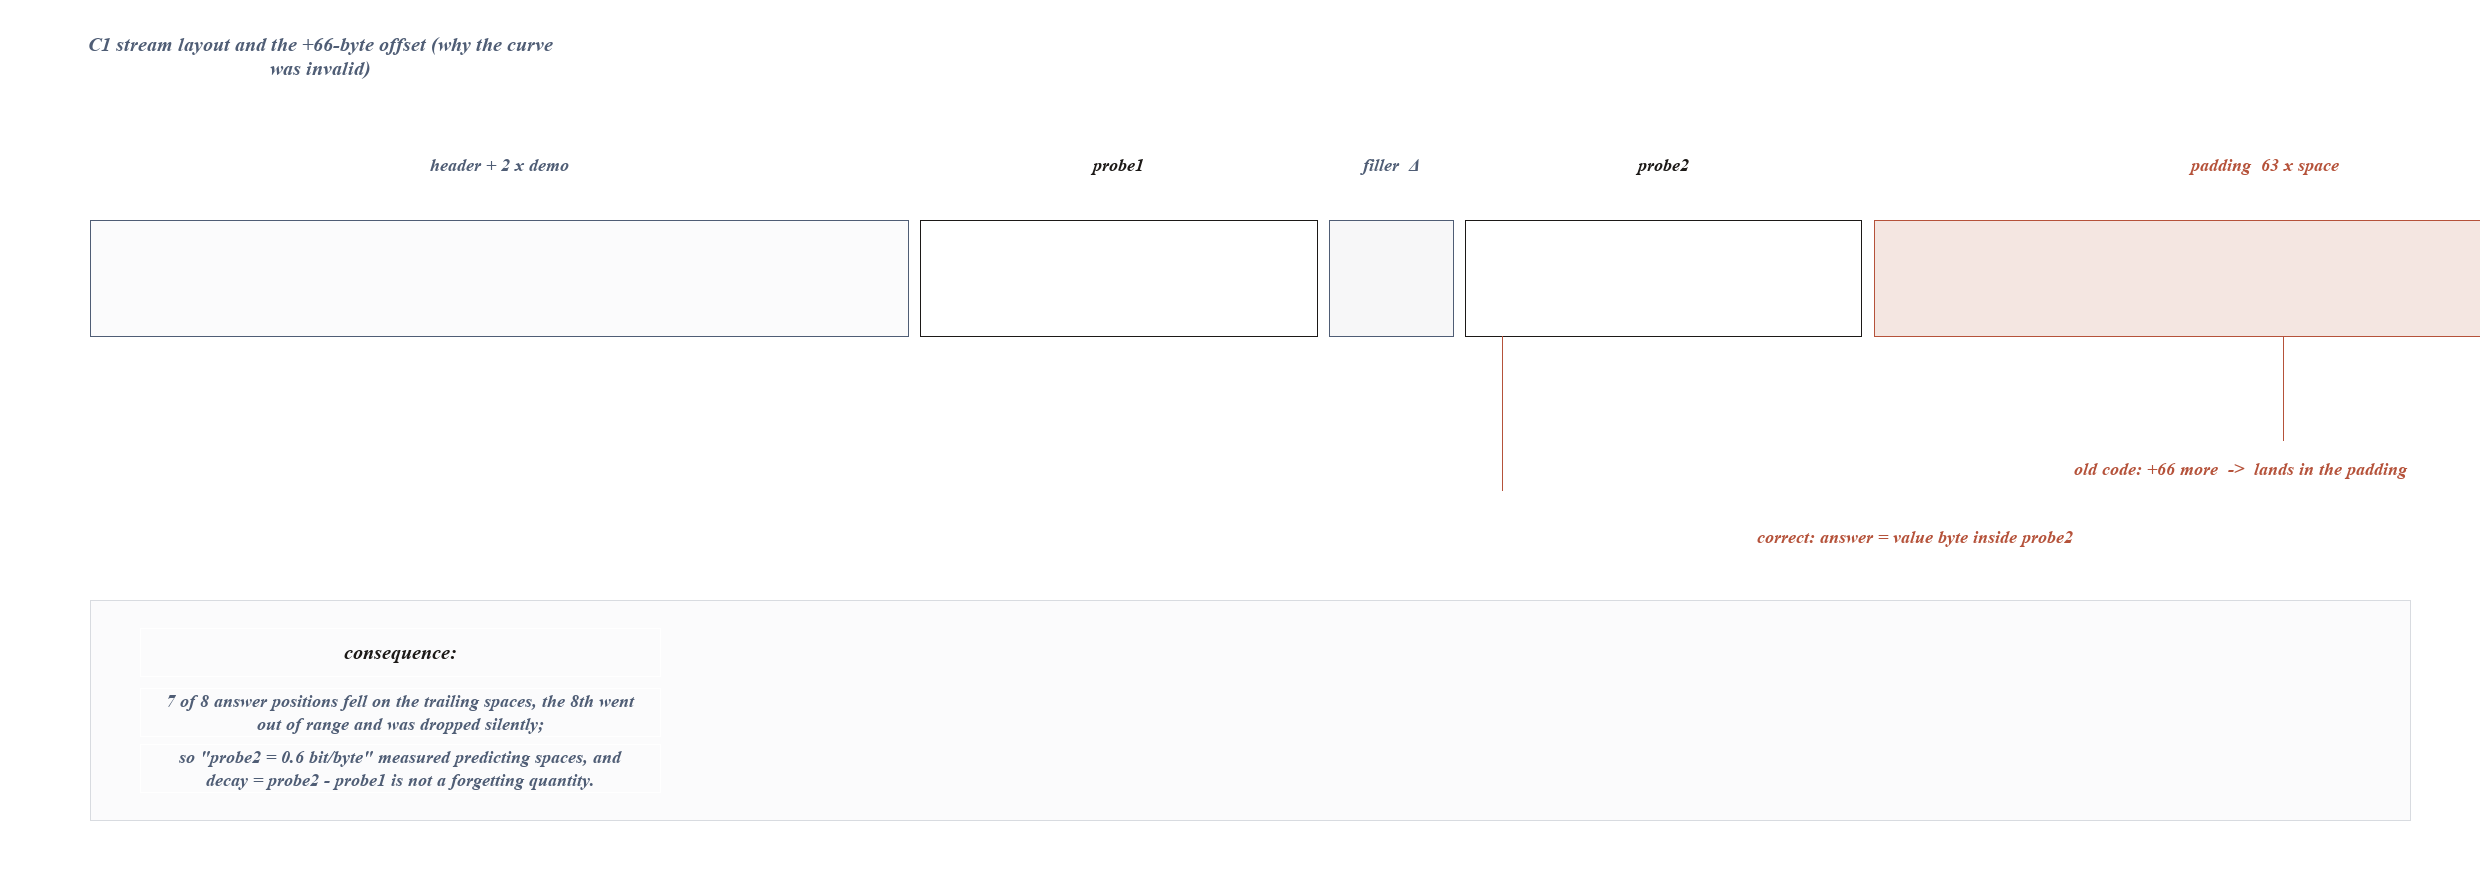
\includegraphics[width=\linewidth]{fig_c1_stream.png}
\caption{C1 的流结构与那 66 字节的偏移（Visio 绘制，源文件 \texttt{figs/fig\_c1\_stream.vsdx}）。
段宽按字节数等比（filler 段压缩），红框为末尾补白；两条竖线分别是「正确答案位置」与「旧代码算出的位置」。}
\label{fig:c1stream}
\end{figure}

\textbf{实验意图。}构造 \texttt{[header $+$ 2$\times$demo $+$ probe1]} $+$ \texttt{filler($\Delta$)}（图 \ref{fig:c1stream}）
$+$ \texttt{probe2} 的合成流（8 对随机 ASCII 键值对、$2$ 次演示），
在 $\Delta\in\{512,2048,8192,32768,131072\}$、$4$ 个条件（正常 / filler 期只读 /
filler 期清零 \texttt{recurrent} / filler 期清零 \texttt{queue}$+$\texttt{MTM}）、$3$ 个 seed 下
测「probe2 相对 probe1 的 recall 衰减」，期望得到按组件分解的遗忘曲线。

\textbf{实测异常。}probe1 的答案位 NLL $=8.38$ bits（机会线 $8.23$），
而 probe2 $=0.6$ bits——\emph{注入后立刻测不会，隔着最多 $128$K token 反而几乎白送}；
四个条件的衰减全挤在 $-7.5$--$-7.8$，彼此不可分。

\textbf{根因（已定位）。}生成脚本把块内偏移基准 $D=\text{header}+2\times\text{demo}=66$ 字节
用在了 probe2 上，而 probe2 的位置又已经叠加了「已注入长度 $+$ $\Delta$」，
于是\textbf{66 字节被算了两次}：8 个答案位置里 7 个落到 probe2 块之后的\textbf{补白空格}上、
第 8 个越界被静默丢弃（代码在位置不在流内时只是跳过）。
所以「probe2 $=0.6$ bits」的真实含义是「模型很会猜一串连续空格」，
而 decay $=$ probe2 $-$ probe1 是伪量。

\textbf{处理。}该实验作废，本文正文不引用其任何数字；
修订版已实现（把「块 $\to$ 答案位置」的算术抽成公共函数，位置一律由「块在流中的绝对起点」推出，
并加断言：答案位置的前一字节必须是 \texttt{=}、后一字节必须是 \texttt{|}），
配套的模型无关自检脚本可在无 GPU 环境下验证位置正确性（旧实现会当场失败）。
\textbf{重跑尚未进行}（预计与原实现同量级，约 80 分钟）。
即使重跑，也需要先注意一个先行事实：本检查点对随机 ASCII 键值对的绑定本身很弱
（附录 \ref{app:g} 的 G1a：$8.3$--$8.6$ bits $\approx$ 机会线），
因此该实验更可能给出「记不住」而不是「记得住但会忘」的结果——
正确的写法是把这类结论归到「离散绑定弱」的机制结论上，而不是包装成遗忘曲线。

\subsection{E2 状态污染与自愈}\label{app:eline}

流结构：正常 8\,KB $+$ 随机字节 4\,KB $+$ 正常 8\,KB；两条件为
\texttt{write\_through}（污染段照常写入）与 \texttt{lock\_garbage}（污染段只读）。
结果见表 \ref{tab:e2} 与图 \ref{fig:e2}：污染段内冲击巨大（$+9.25$ / $+9.92\nats$），
但两组条件的尾值与残留几乎相同（$0.8608$ vs $0.8607$；$+0.085$ vs $+0.085\nats$），
污染后前 4 个 patch 才有明显差异（$0.686$ vs $0.436\nats$）。
\textbf{结论}：污染写入造成瞬时冲击、无长期残留；「只读模式作为污染防御」得不到数据支持。
尾部相对基线的 $+0.085\nats$ 抬升更可能来自文本难度漂移（与 \S\ref{sec:b1} 的 E5 判据一致）。

\begin{table}[H]
\centering
\caption{E2 污染与自愈（nats）。恢复长度按「回到基线 $+0.5$ 以内」判定。}
\label{tab:e2}
\small
\begin{tabular}{@{}lcccccc@{}}
\toprule
条件 & 污染前 & 污染段内 & 污染后 4 patch & 尾部 & 残留 & 恢复（patch） \\
\midrule
write\_through & $0.776$ & $10.027$ & $0.686$ & $0.861$ & $+0.085$ & $0$ \\
lock\_garbage & $0.776$ & $10.696$ & $0.436$ & $0.861$ & $+0.085$ & $0$ \\
\bottomrule
\end{tabular}
\end{table}

\begin{figure}[H]
\centering
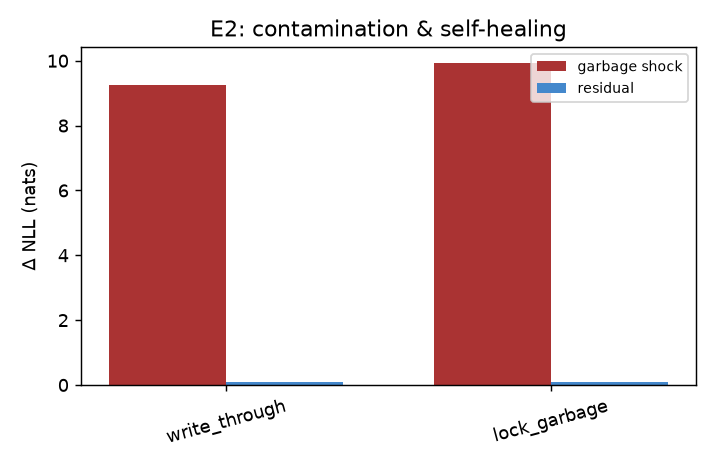
\includegraphics[width=0.62\linewidth]{fig_e2_contamination.png}
\caption{E2：污染段的冲击与残留。冲击量级远大于残留，且两条件的残留相同。}
\label{fig:e2}
\end{figure}

\section{D 线与 G 线的完整数字}\label{app:dline}\label{app:g}

\begin{table}[H]
\centering
\caption{G 线前向学习：合成任务与自然语料。指标为答案位 NLL 的均值（bits），
$5$ 个 seed 的 95\% CI；write / lock 两条件。数值越大越差，机会线见表内注。}
\label{tab:g}
\small
\begin{tabular}{@{}llcc@{}}
\toprule
任务 & 设定 & write & lock \\
\midrule
G1a 随机 ASCII 键值对联想 & $k=0$（无演示） & $8.93\pm0.62$ & $8.93\pm0.62$ \\
（机会线 $\log_2 85\approx6.4$ bits） & $k=1$ & $7.54\pm0.49$ & $7.54\pm0.49$ \\
 & $k=2$ & $8.31\pm0.34$ & $8.98\pm0.65$ \\
 & $k=8$ & $8.53\pm0.61$ & $8.98\pm0.65$ \\
 & $k=16$ & $8.61\pm0.72$ & $8.98\pm0.65$ \\
\midrule
G1b 单字节 bigram 转移 & $k\le8$ & $\approx3.6$--$3.9$ & 同 write \\
（CI 很大，仅定性） & $k=16$ & $3.15\pm1.82$ & $3.91\pm2.21$ \\
 & $k=32$ & $3.33\pm1.96$ & $3.91\pm2.21$ \\
\midrule
G1c 分布内高频词对联想 & $k=0$ & $5.15\pm0.31$ & $5.34\pm0.58$ \\
 & $k=8$ & $4.96\pm0.14$ & $5.17\pm0.30$ \\
 & $k=16$ & $5.19\pm0.12$ & $5.24\pm0.43$ \\
\midrule
G2 自然语料 $\mathrm{8}$-gram 复现 & 首次 / 二次（nats） & $0.732\to0.678$ & $1.483\to1.499$ \\
（32\,KB，3382 对，间距 $<\!4$k） & 增益 (nats) & $\mathbf{+0.054}$ & $-0.016$ \\
\bottomrule
\end{tabular}
\end{table}

\begin{figure}[H]
\centering
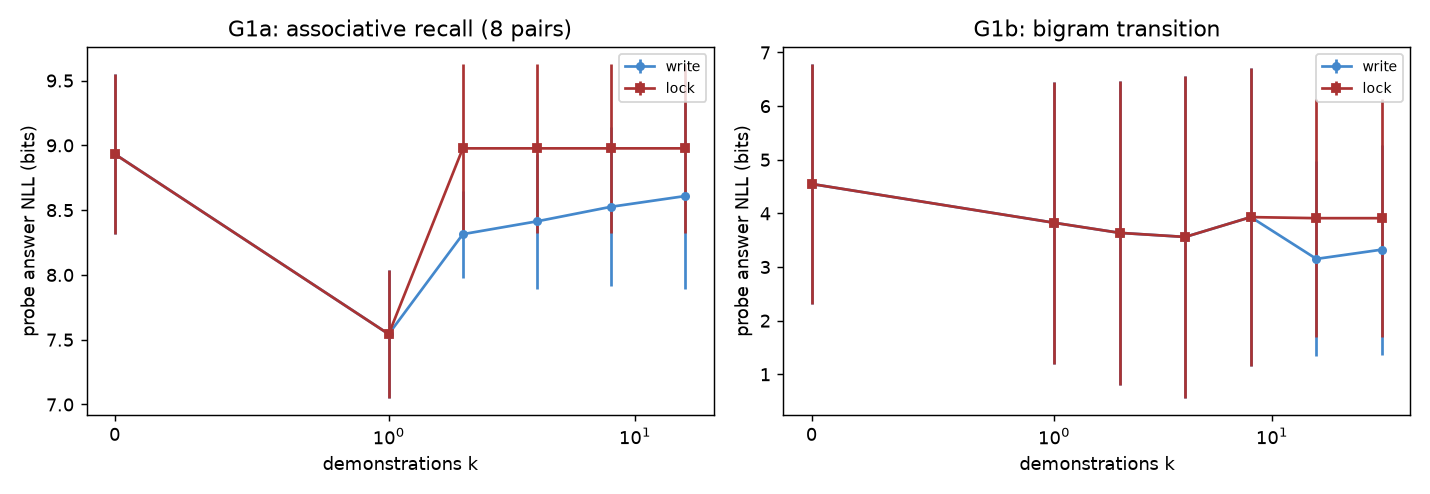
\includegraphics[width=\linewidth]{fig_g1_forward_learning.png}
\caption{G1a / G1b：前向学习曲线（$k$ 为演示次数）。联想任务上 write 曲线不随 $k$ 累积；
bigram 任务需要 $k\ge16$ 才出现跨 patch 效应，且置信区间极大。}
\label{fig:g1}
\end{figure}

\begin{figure}[H]
\centering
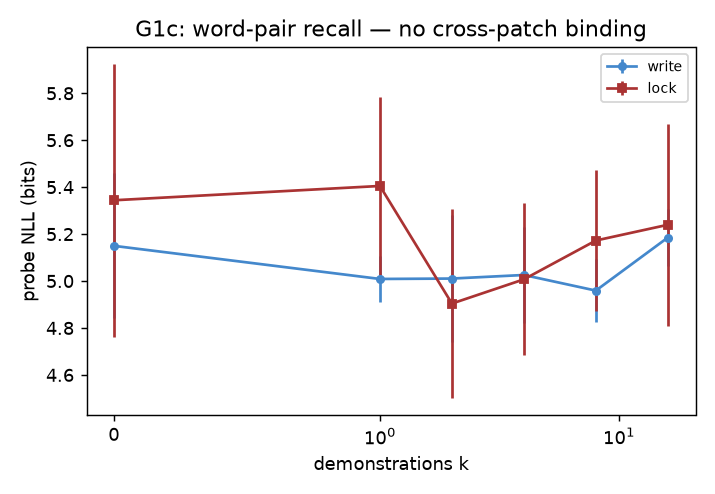
\includegraphics[width=0.62\linewidth]{fig_g1c_word_assoc.png}
\caption{G1c：把符号换成分布内高频词对后曲线依然全平（$\approx$ 首字节机会线），
排除「随机 ASCII 太 OOD」这一解释。}
\label{fig:g1c}
\end{figure}

\begin{figure}[H]
\centering
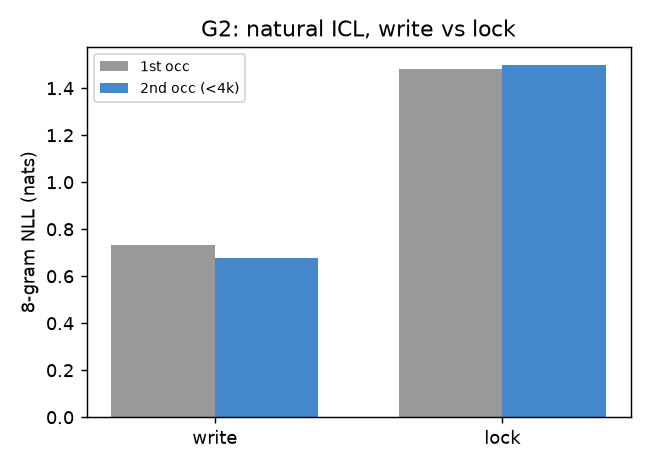
\includegraphics[width=0.55\linewidth]{fig_g2_natural_icl.png}
\caption{G2：自然语料 $8$-gram 的二次出现增益 $+0.054\nats$，且在 $\mathit{lock}$ 下消失——
说明该增益是写入依赖的、且量级很小。}
\label{fig:g2}
\end{figure}

\section{F 线与 H 线：未运行}\label{app:f-h}

F 线（训练动力学）需要重训，超出「只用现成权重」的范围：
BPTT 窗口扫描、永续 vs 文档边界重置、状态统计演化、\texttt{chunk\_size} 扫描、状态收敛时间。
H 线（任务级 demo：多会话一致性、长文档跨块一致性、代码跨文件一致性）依赖推理链冻结后再做。
两项都按 \S\ref{sec:f-line} 的优先级排序，本稿不给任何推测数值。
